%%%%%%%%%%%%%%%%%%%%%%%%%%%%%%%%%%%%%%%%%%%%%%%%%%%%%%%%%%%%%%%%%%
%%%%%%%%			PRIOR ART
%%%%%%%%%%%%%%%%%%%%%%%%%%%%%%%%%%%%%%%%%%%%%%%%%%%%%%%%%%%%%%%%%%

\subsection{Prior Art}

\paragraph{}
For a thorough research project to be completed, devices that have already been designed, tested and created must be research and analysed. With the popularity of DC power systems increasing in recent years, there have been an many more academics assessing the possibilities. Due to the predominately theoretical design nature of this report and similar aspects of previous papers, a significant focus was made on previous papers.  

\subsubsection{Previous Thesis: Extra-Low Voltage In-Home Power Distribution and Storage}

\paragraph{}
Steven Donohue completed his undergraduate thesis under Geoffery Walker in 2014 \cite{Donohue2014}. This paper assessed various aspects of the similar topic question but specifically focussed on using low voltage DC electricity in homes to power lighting systems. He also considered battery storage solutions and devised that 48V was the best option for voltage levels for this application \cite{Donohue2014}. He finalised that a proposed installation model for low voltage distribution was uneconomical with current solar feed-in tariffs \cite{Donohue2014}. The final discussion of lighting application proved to be successful using LED lighting circuits in home. Donohue's project will be an asset to the completion of this thesis as the overall concept is very similar. It will be possible to make some assumptions and avoid investing time on smaller calculations due to Donohue's extensive research.         

\subsubsection{Previous Thesis: DC Supply In Buildings}

\paragraph{}
From the University of Science and Technology in Norway, Aurora Bøhle Foss completed her master's thesis on encorporating DC supply into buildings with a larger focus on commercial buildings \cite{Foss2014}. Her focus wasn't specifically to do with low voltage DC however it did incorporate some research and testing into the feasibility of these systems. her research found that the most important aspect of incorporating DC supplies into power systems is a highly efficient Voltage Source Converter (VSC). She discovered that if a load is requiring AC, it is more efficient to use an AC source. It has been found that higher power loads and cable lengths longer than 10 metres using  $1.5\text{mm}^{2}$ and  $2.5\text{mm}^{2}$ are impossible due to severe losses.

\subsubsection{Micro-Inverters}

\paragraph{}
A competitor to the system that will be designed throughout this thesis will be recent developments in micro-inverter technologies by Enphase \cite{website:Enphase}. These products are designed to be efficient, small and affordable to allow for the DC electricity generated by photo-voltaic cells to be converted to 240V 50Hz AC for the mains. A wide range of fittings are possible depending on the PV cells and switchboard distribution. They have a rated efficiency of 95.7\% \cite{website:Enphase}.       

\subsubsection{EP 0516025A3 Low Voltage DC to DC Converter}

\paragraph{}
Due to this project being predominately simulation based and not specifically building an improved system, it will need to consider existing devices. As discussed, the largest hurdle will be ensuring that the devices maintain a high enough efficiency to allow DC systems to be viable. This patent represents the construction of a low voltage DC converter utilising MOSFETs \cite{Hulsey1992}. The figure below shows the circuit diagram patented. 

\begin{figure}[H]
\hfill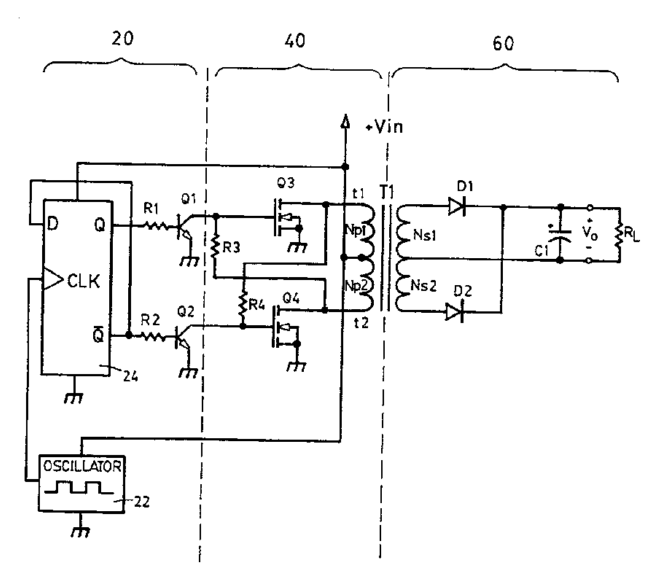
\includegraphics[width = 100mm]{images/DC_Conv_Patent}\hspace*{\fill}
\caption{Low Voltage DC to DC Converter Design Patent \cite{Hulsey1992}}
\label{fig:DC2DC}
\end{figure}

\subsubsection{US 7435897B2 Apparatus and Method For Mounting Photovoltaic Power Generating Systems on Buildings}

\paragraph{}
Miles Russell from Schott Solar, Inc based out of Massachusetts developed a new apparatus for mounting PV systems onto larger buildings \cite{Russes2002}. It is not as technical but it discusses the benefits of utilising a specific mounting system for the largest energy production. The design is a simpler way of implementing the physical connection of panels to larger buildings. This patent does not consider the inverters or circuitry, it is purely for the attachment and orientation of panels.   
\newpage